\documentclass[10pt]{beamer}

\usetheme[progressbar=frametitle]{metropolis}
% \usepackage{appendixnumberbeamer}

% \usepackage{booktabs}
% \usepackage[scale=2]{ccicons}

% \usepackage{pgfplots}
% \usepgfplotslibrary{dateplot}

% \usepackage{xspace}
% \newcommand{\themename}{\textbf{\textsc{metropolis}}\xspace}

\title{MTH 201: Calculus -- Module 1B}
\subtitle{The concept of the limit (AC 1.2)}
% \date{\today}
\date{}
\author{Robert Talbert}
\institute{Grand Valley State University}
% \titlegraphic{\hfill\includegraphics[height=1.5cm]{logo.pdf}}

\begin{document}

\maketitle

\begin{frame}{Agenda}
  \setbeamertemplate{section in toc}[sections numbered]
  \tableofcontents%[hideallsubsections]
\end{frame}





\section[Review of Daily Prep]{Daily Prep Review}

\begin{frame}{Polling for today}

\large{
Go to \textbf{\url{www.mentimeter.com}} and enter code \texttt{32 04 90} 
\vskip
Or  go to \url{https://www.menti.com/4d48wn64k6}}
\end{frame}

\section[Q+A]{Q+A from Daily Prep}

\section[Limits using algebra]{Limits using algebra}

\begin{frame}{Finding limits using algebra}
    \metroset{block=fill}
      \begin{alertblock}{Alert}
        \textbf{Finding a limit of a function at a point, is not always the same thing as evaluating the function at that point.}
      \end{alertblock}
      
     \begin{exampleblock}{Example}
     \begin{equation*}
         \lim_{x \to 2} \frac{x^2-4}{x-2} = 4
     \end{equation*}
    \begin{center}
             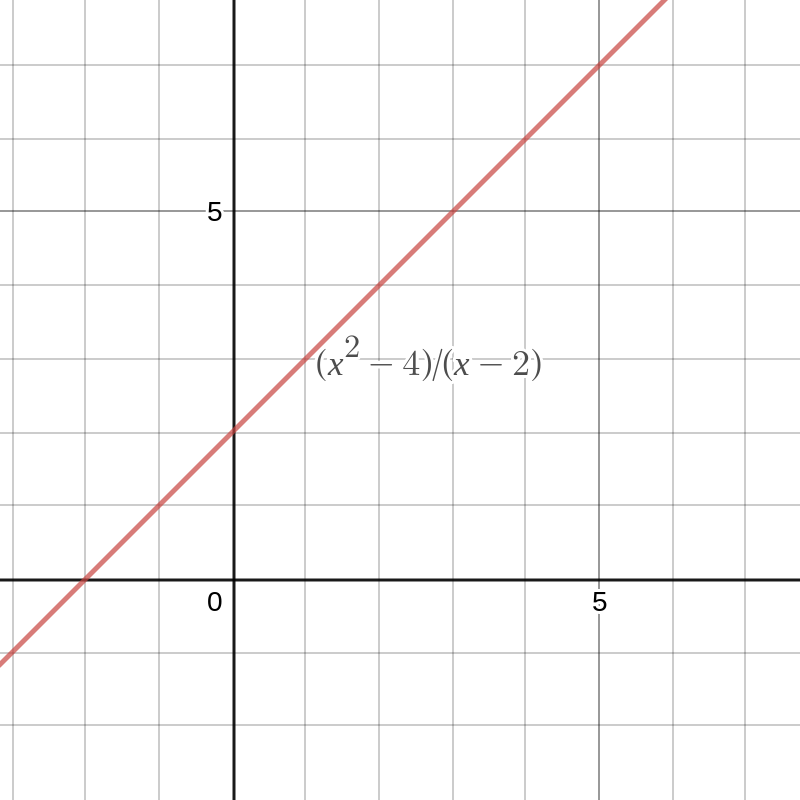
\includegraphics[width=1.25in]{1b-in-1.png}
    \end{center}
         But $\frac{x^2 - 4}{x-2}$ evaluated at $x=2$ is undefined ($0/0$). 
     \end{exampleblock}
\end{frame}

\begin{frame}{Using algebra first}
    \metroset{block=fill}
    \begin{block}{Pro Tip}
    Always try to simplify the algebra first. 
    \end{block}
    
    \begin{exampleblock}{Example}
     \begin{align*}
         \lim_{x \to 2} \frac{x^2-4}{x-2} &= \lim_{x \to 2} \frac{(x-2)(x+2)}{x-2} \\
         &= \lim_{x \to 2} (x+2)
     \end{align*}
    As $x$ gets closer to $2$, $x+2$ gets closer to $4$. \vskip
    
    Therefore $\lim_{x \to 2} \frac{x^2-4}{x-2} = 4$.
        \end{exampleblock}
\end{frame}

\begin{frame}{Practice with the concept}
    
    Go to: 
    
    \begin{center}
        \url{http://gvsu.edu/s/1pq}
    \end{center}
    
Find the value of the limit using algebra simplification first. 

\begin{itemize}
    \item $(x+2)^3$ does not equal $x^3 + 8$
    \item The answer is 12. 
\end{itemize}
    
\end{frame}

\section[Instantaneous velocity using limits]{Instantaneous velocity using limits}

\begin{frame}{Average velocity}

Consider a moving object whose position function is given by $s(t) = t^2$ where $t$ is time in seconds, $s$ is position in meters. 

\begin{center}
    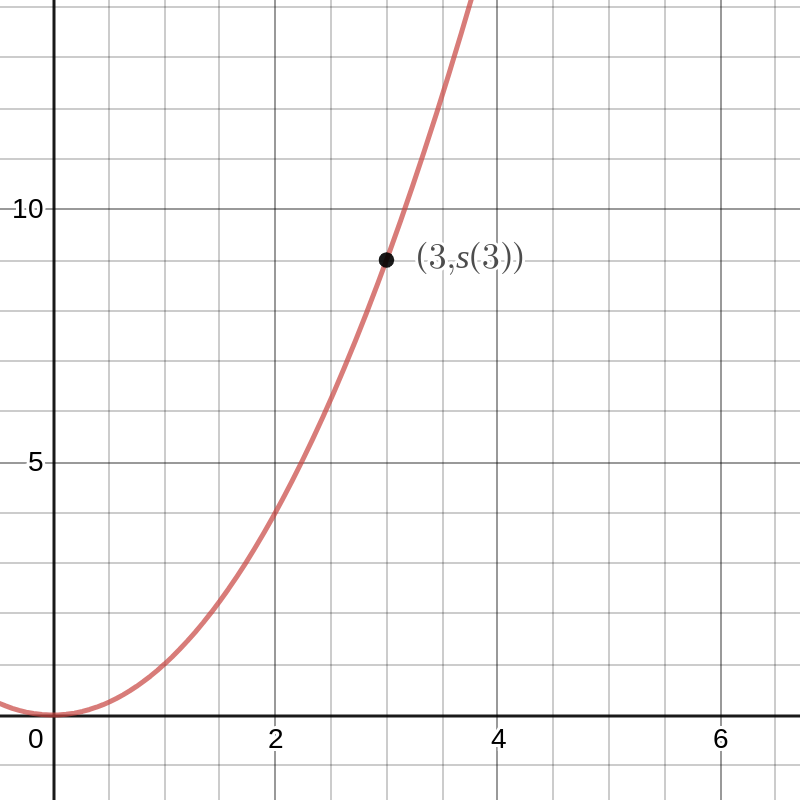
\includegraphics[width=2in]{1b-in-2.png}
\end{center}

\end{frame}

\begin{frame}{Finding average and instantaneous velocity}

The \textbf{average velocity} on the small time interval from $t=3$ to $t=3+h$ is
\begin{equation*}
    \frac{s(3+h)-s(3)}{(3+h)-3} = \frac{s(3+h) - s(3)}{h}
\end{equation*}

On Mentimeter: If we wanted to find the \textit{instantaneous velocity} at $t=3$, how would we modify this? 
    
\end{frame}

\begin{frame}{Working out the velocity}
    We get the instantaneous velocity at $t=3$ by taking the \textbf{average velocity} expression and \textbf{evaluating its limit as $h \to 0$}: 
    
    \begin{equation*}
        IV_{t=3} = \lim_{h \to 0} \frac{s(3+h) - s(3)}{h}
    \end{equation*}
    
But we can now work out the value with algebra! Work with your partner to do this: 
    \begin{center}
        \url{http://gvsu.edu/s/1pt}
    \end{center}

Spoiler: The answer is 6 meters/second. 
\end{frame}

\begin{frame}{Getting the instantaneous velocity}
\begin{align*}
    IV_{t=3} &= \lim_{h \to 0} \frac{s(3+h) - s(3)}{h} \\
    &= \lim_{h \to 0} \frac{(3+h)^2 - 9}{h} \\
    &= \lim_{h \to 0} \frac{9 + 6h + h^2 - 9}{h} \\
    &= \lim_{h \to 0} \frac{6h + h^2}{h} \\
    &= \lim_{h \to 0} \frac{h(6 + h)}{h} \\
    &= \lim_{h \to 0} (6+h) \\
    &= 6 \ \text{meters/second}
\end{align*}

\end{frame}

\section[What to do next]{What to do next}
\begin{frame}{Coming up next}
    \begin{itemize}
    \item Online followup activities: Due 11:59pm ET, Friday 9/11 (Link to be posted and in email) 
    \item Daily Prep for Module 2A: Due 11:59pm ET, Sunday 9/13 (Blackboard)
    \item WeBWorK 1B: Due 11:59pm ET, Sunday 9/13 (WeBWorK)
\end{itemize}

\textbf{Continue to check email and announcements every day --- ask questions and give help on CampusWire too.}

\vfill
\begin{center}\ccbysa\end{center}

\end{frame}


\end{document}
